\subsection{Concentration with 64 responses per prompt}
\label{app:fresh-concentration}

We evaluate initial and terminal checkpoints on the 128 held-out Level-1
\texttt{Graph} and \texttt{PantryPlan} prompts, drawing 64 responses per
prompt from new sampling streams. This evaluation is separate from the
32-response comparison in Fig.~\ref{fig:concentration-story}. It covers
Qwen2.5-0.5B, Falcon3-1B, and Qwen2.5-3B, with five training seeds for
Dr.GRPO, Re:Dr, MaxRL, and Re:Max. For each model, the five initial
evaluations use independent sampling from the same weights. Each initial
evaluation is paired with one training seed and shared across the four methods.

\paragraph{Matched comparisons.}
We estimate \pmd{} from correct-output pairs and average promptwise
differences over prompts with at least two correct responses in both
conditions, then average the five seed effects equally. Thus positive
changes indicate more diverse correct modes. Matching prompts within each
comparison differs from subtracting means over separately eligible prompts.
The eligible population ranges from 37 to 127 of the 128 prompts across
comparisons and seeds. Effects from different comparisons therefore cannot
be subtracted to reconstruct a trajectory on a common prompt population. Tables~\ref{tab:fresh-concentration-initial}
and~\ref{tab:fresh-concentration-replay} give all 36 contrasts and their
eligible-prompt ranges. Intervals are nominal 95\% paired Student-$t$
intervals with four degrees of freedom. They describe variation over the
five training-seed and initial-sampling pairs, conditional on the fixed
prompts and initial weights. They are unadjusted for multiple comparisons
and do not quantify uncertainty over unseen tasks.

\begin{figure}[t]
 \centering
 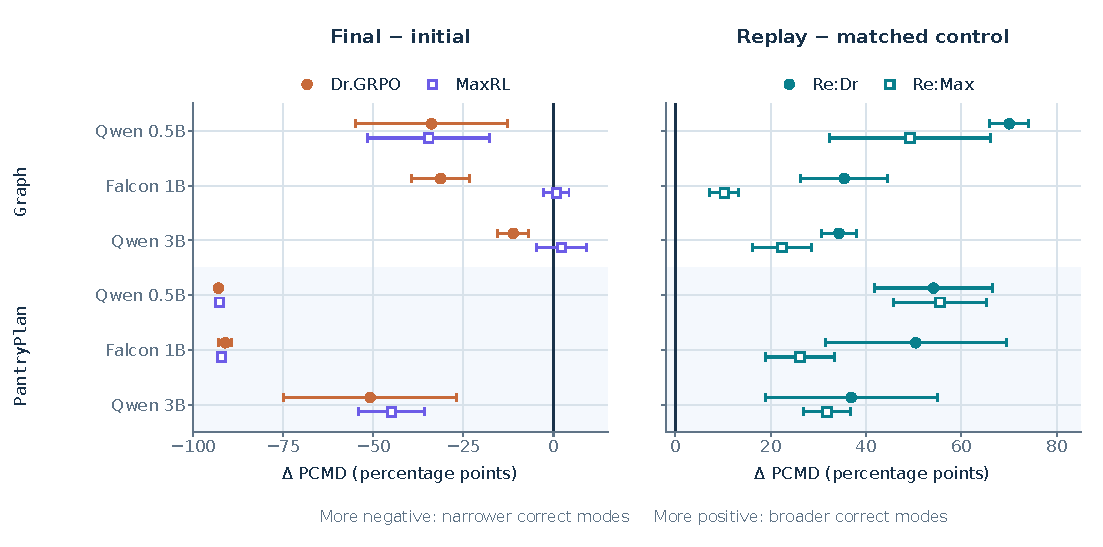
\includegraphics[width=\linewidth]{figures/fresh_concentration_pcmd_20260912.pdf}
 \caption{\textbf{Replay increases correct-mode diversity at a 64-response budget.}
 Left: Dr.GRPO reduces \pmd{} in all six model--domain comparisons;
 MaxRL's change is inconclusive for Falcon3-1B and Qwen2.5-3B \texttt{Graph}.
 Right: replay increases \pmd{} in all twelve comparisons with matched
 trained controls. Points show means over five paired seeds; bars give
 nominal 95\% Student-$t$ intervals. Each contrast uses its own jointly
 eligible Level-1 prompts. Horizontal scales differ between panels.}
 \label{fig:fresh-concentration}
\end{figure}

\paragraph{Concentration and mitigation.}
Dr.GRPO reduces \pmd{} in all six model--domain comparisons and all
30 seed effects. Replay increases \pmd{} relative to its matched trained
control under both objectives in all twelve comparisons and all 60 seed
effects. All eighteen nominal intervals exclude zero
(Fig.~\ref{fig:fresh-concentration}). These directions also hold when
pooling correct pairs, using each policy's own eligible prompts, or
restricting to the intersection of eligible prompts across seeds.
The intersection can be small: for Qwen2.5-0.5B \texttt{Graph}, only five
prompts are jointly eligible across all seeds in comparisons involving Dr.GRPO.

MaxRL alone does not consistently reduce diversity: its Falcon3-1B and
Qwen2.5-3B \texttt{Graph} intervals include zero. An improvement over a
trained control also need not restore initial diversity. Both replay
variants remain below initial \pmd{} in \texttt{PantryPlan} at every
scale, whereas their \texttt{Graph} comparisons exceed the initial value.
These results describe diversity within each comparison's eligible prompt
population; they do not establish recovery of the same individual modes.

\paragraph{Correctness, coverage, and sampling budget.}
All 24 trained-versus-initial comparisons increase per-response
correctness averaged over all evaluation prompts, in every seed. Nevertheless, every
\texttt{PantryPlan} method--scale comparison has lower \texttt{pass@64}
than initialization in every seed. Averaging over all evaluation prompts,
replay improves mean
\texttt{pass@8}, \texttt{distinct@8}, \texttt{pass@64}, and
\texttt{distinct@64} relative to its trained control in all twelve
comparisons; per-response correctness improves in seven of twelve.
On jointly eligible prompts, however, replay lowers mean correctness in
eleven of twelve comparisons. The concentration effects therefore do not
hold correctness fixed.

The eight-response metrics average over subsets of eight responses from
each 64-response pool (rarefaction). For Qwen2.5-3B \texttt{Graph}, Dr.GRPO increases per-response correctness by
14.49 percentage points and \texttt{distinct@8} by 0.112 modes per prompt,
while reducing \pmd{} by 11.20 points and \texttt{distinct@64} by
0.220 modes. The change in verified-mode count reverses sign between
eight and 64 responses in every seed. A gain at one sampling budget thus
need not persist at a larger budget. These evaluations measure the
distribution of correct responses and the modes observed in finite samples;
they do not establish exact mode extinction, recovery of the full support,
or a causal effect of diversity on accuracy.

% Generated by ops/build_paper_fresh_concentration.py; do not hand edit.
\begin{table}[t]
\centering
\small
\setlength{\tabcolsep}{4pt}
\caption{64-response evaluation: trained policy minus initialization. Changes in \pmd{} are in probability units; positive values indicate more diverse correct modes. Brackets give nominal 95\% paired Student-$t$ intervals ($n=5$, four degrees of freedom). The last column gives the range of jointly eligible prompts across seeds, out of 128. Each row uses its own matched prompt population.}
\label{tab:fresh-concentration-initial}
\begin{tabular}{llrr}
\toprule
Domain & Contrast & $\Delta\pmd$ [95\% interval] & Joint prompts \\
\midrule
\multicolumn{4}{l}{\textbf{Qwen2.5-0.5B}} \\
\texttt{Graph} & Dr.GRPO $-$ initial & $-0.338\;[-0.550, -0.126]$ & 37--45 \\
 & Re:Dr $-$ initial & $+0.217\;[+0.190, +0.243]$ & 97--103 \\
 & MaxRL $-$ initial & $-0.346\;[-0.516, -0.177]$ & 37--86 \\
 & Re:Max $-$ initial & $+0.155\;[+0.107, +0.203]$ & 97--101 \\
\texttt{PantryPlan} & Dr.GRPO $-$ initial & $-0.929\;[-0.936, -0.923]$ & 62--68 \\
 & Re:Dr $-$ initial & $-0.357\;[-0.445, -0.269]$ & 109--122 \\
 & MaxRL $-$ initial & $-0.927\;[-0.932, -0.921]$ & 62--71 \\
 & Re:Max $-$ initial & $-0.355\;[-0.438, -0.272]$ & 108--124 \\
\midrule
\multicolumn{4}{l}{\textbf{Falcon3-1B}} \\
\texttt{Graph} & Dr.GRPO $-$ initial & $-0.313\;[-0.393, -0.233]$ & 75--99 \\
 & Re:Dr $-$ initial & $+0.043\;[+0.006, +0.081]$ & 100--107 \\
 & MaxRL $-$ initial & $+0.008\;[-0.027, +0.043]$ & 104--109 \\
 & Re:Max $-$ initial & $+0.119\;[+0.096, +0.141]$ & 106--109 \\
\texttt{PantryPlan} & Dr.GRPO $-$ initial & $-0.910\;[-0.928, -0.893]$ & 81--86 \\
 & Re:Dr $-$ initial & $-0.378\;[-0.507, -0.250]$ & 104--110 \\
 & MaxRL $-$ initial & $-0.921\;[-0.925, -0.916]$ & 81 \\
 & Re:Max $-$ initial & $-0.519\;[-0.575, -0.462]$ & 106--116 \\
\midrule
\multicolumn{4}{l}{\textbf{Qwen2.5-3B}} \\
\texttt{Graph} & Dr.GRPO $-$ initial & $-0.112\;[-0.156, -0.069]$ & 78--86 \\
 & Re:Dr $-$ initial & $+0.226\;[+0.212, +0.240]$ & 88--96 \\
 & MaxRL $-$ initial & $+0.022\;[-0.048, +0.092]$ & 81--93 \\
 & Re:Max $-$ initial & $+0.254\;[+0.234, +0.274]$ & 90--96 \\
\texttt{PantryPlan} & Dr.GRPO $-$ initial & $-0.509\;[-0.750, -0.268]$ & 69--99 \\
 & Re:Dr $-$ initial & $-0.115\;[-0.157, -0.073]$ & 101--110 \\
 & MaxRL $-$ initial & $-0.449\;[-0.541, -0.358]$ & 83--98 \\
 & Re:Max $-$ initial & $-0.116\;[-0.208, -0.024]$ & 105--110 \\
\bottomrule
\end{tabular}
\end{table}

% Generated by ops/build_paper_fresh_concentration.py; do not hand edit.
\begin{table}[t]
\centering
\small
\setlength{\tabcolsep}{4pt}
\caption{64-response evaluation: replay minus its matched trained control. Changes in \pmd{} are in probability units; positive values indicate more diverse correct modes. Brackets give nominal 95\% paired Student-$t$ intervals ($n=5$, four degrees of freedom). The last column gives the range of jointly eligible prompts across seeds, out of 128. Each row uses its own matched prompt population.}
\label{tab:fresh-concentration-replay}
\begin{tabular}{llrr}
\toprule
Domain & Contrast & $\Delta\pmd$ [95\% interval] & Joint prompts \\
\midrule
\multicolumn{4}{l}{\textbf{Qwen2.5-0.5B}} \\
\texttt{Graph} & Re:Dr $-$ Dr.GRPO & $+0.700\;[+0.659, +0.742]$ & 40--46 \\
 & Re:Max $-$ MaxRL & $+0.493\;[+0.324, +0.662]$ & 41--107 \\
\texttt{PantryPlan} & Re:Dr $-$ Dr.GRPO & $+0.542\;[+0.418, +0.665]$ & 62--68 \\
 & Re:Max $-$ MaxRL & $+0.555\;[+0.458, +0.652]$ & 61--71 \\
\midrule
\multicolumn{4}{l}{\textbf{Falcon3-1B}} \\
\texttt{Graph} & Re:Dr $-$ Dr.GRPO & $+0.354\;[+0.264, +0.445]$ & 73--101 \\
 & Re:Max $-$ MaxRL & $+0.103\;[+0.072, +0.133]$ & 122--127 \\
\texttt{PantryPlan} & Re:Dr $-$ Dr.GRPO & $+0.505\;[+0.315, +0.694]$ & 80--84 \\
 & Re:Max $-$ MaxRL & $+0.262\;[+0.190, +0.334]$ & 81 \\
\midrule
\multicolumn{4}{l}{\textbf{Qwen2.5-3B}} \\
\texttt{Graph} & Re:Dr $-$ Dr.GRPO & $+0.343\;[+0.307, +0.380]$ & 94--107 \\
 & Re:Max $-$ MaxRL & $+0.224\;[+0.163, +0.286]$ & 105--123 \\
\texttt{PantryPlan} & Re:Dr $-$ Dr.GRPO & $+0.369\;[+0.188, +0.550]$ & 72--101 \\
 & Re:Max $-$ MaxRL & $+0.319\;[+0.270, +0.367]$ & 89--99 \\
\bottomrule
\end{tabular}
\end{table}

\FloatBarrier
